\section{Motivation}\label{sec:motiv}
In this section, we first discuss existing research achievements in
the pursuit of formally defining object-oriented languages with symmetric
multiple dispatch, multiple inheritance, and parametric polymorphism with
variance.  Then, we present how FGFV completes the long-standing endeavor
by defining a core calculus with static overloading rules and a dynamic
dispatch algorithm that are proven type-sound.

\subsection{Overloading Rules for Multiple Inheritance}\label{sec:motiv:ff}
As we discussed in Section~\ref{sec:intro}, both symmetric multiple
dispatch and multiple inheritance may cause ambiguous method calls
that cannot be resolved at run time.  Let us assume that class $C$ is the only
subtype of both classes $A$ and $B$, and they are all distinct
throughout this section.  Consider
the following overloaded method declarations of $m_1$:
\[\begin{array}[ht]{l@{\hskip2em}l}
\hbox to 12 em{$m_1(x \COLON B, y \COLON C) \COLON B = \cdots$\hfil} & 
\hbox to 12 em{$m_1(x \COLON C, y \COLON B) \COLON B = \cdots$\hfil}
\end{array}\]
which have the same return type $B$ but different domain types
$\tuple{B,C}$ and $\tuple{C,B}$.  For a method invocation $m_1(c, c)$
where the run-time type of $c$ is $C$, it is ambiguous which declaration
to invoke due to symmetric multiple dispatch: both method declarations
are applicable to $(c, c)$ since both $\tuple{B,C}$ and $\tuple{C,B}$ are
supertypes of $\tuple{C,C}$, and neither declaration is more specific
than the other.  Also, consider the following overloaded declarations of
$m_2$:
\[\begin{array}[ht]{l@{\hskip2em}l}
\hbox to 12 em{$m_2(x \COLON A) \COLON \TYP{Boolean} = \cdots$\hfil} &
\hbox to 12 em{$m_2(x \COLON B) \COLON \TYP{Boolean} = \cdots$\hfil}
\end{array}\]
which have domain types $A$ and $B$, respectively.  For a method invocation $m_2(c)$,
it is ambiguous which declaration to invoke due to multiple inheritance:
both declarations are applicable to $c$ and neither declaration is more
specific than the other.

In order to guarantee that no such ambiguous method calls are possible
at run time, researchers have proposed several calculi with restrictions
on overloaded method declarations.  CF~\cite{ff}, Core Fortress, is a core
calculus of the Fortress programming language~\cite{fortress}, which contains
components, top-level functions, functional methods, and declarations
of exclusive types in addition to multiple inheritance.  However, it
does not specify the language semantics and informally provides rules
for valid overloaded method declarations.  FFMM~\cite{ffcoq},
Featherweight Fortress with Multiple Dispatch and Multiple Inheritance,
simplified CF to focus only on multiple inheritance, and it has a
complete formalization of the language semantics including overloading
rules and its type soundness proof in Coq.  Since the overloading rules
of CF and FFMM are the same, we will refer to these two languages collectively as
\textit{Featherweight Fortress (FF)}.

The overloading rules of FF require every pair in a set of overloaded
method declarations to satisfy \emph{one} of the following rules:
\begin{description}
\item[\textbf{Exclusion Rule:}] Their domain types are \textit{exclusive}
(their intersection is $\Bottom$, where the $\Bottom$ type is a subtype of every type and
no value belongs to $\Bottom$).

\item[\textbf{Subtype Rule:}] The domain type of one declaration is
a strict subtype of the domain type of the other, and the return type of
the former is a subtype of the return type of the latter.

\item[\textbf{Meet Rule:}] The domain types are not exclusive nor in a
subtype relation, and the overloaded set contains a third disambiguating
method declaration which we call the \textit{meet} of the pair.
The meet of two method declarations is more specific than each of the
declarations and less specific than any other method declaration that is
more specific than both declarations.
\end{description}

Let us revisit the previous examples, with an additional
method declaration each for $m_1$ and $m_2$:
\[
\begin{array}[ht]{@{}l@{$\;$}l@{$\;$}l@{\hskip2.5em}l@{$\;$}l@{$\;$}l@{\hskip2.5em}l@{$\;$}l@{$\;$}l}
d_1^1:\ m_1(x \COLON B, y \COLON C) \COLON B &=& \cdots 
& d_1^2:\ m_1(x \COLON C, y \COLON B) \COLON C &=& \cdots 
& d_1^3:\ m_1(x \COLON C, y \COLON C) \COLON C &=& \cdots \\
d_2^1:\ m_2(x \COLON A) \COLON \TYP{Boolean} &=& \cdots
& d_2^2:\ m_2(x \COLON B) \COLON \TYP{Boolean} &=& \cdots
& d_2^3:\ m_2(x \COLON C) \COLON \TYP{Boolean} &=& \cdots
\end{array}\]
Note that, for both $m_1$ and $m_2$, the third method declaration is the
meet of the first two declarations.
% Each set of overloaded method
% declarations is valid since every pair satisfies one of the overloading
% rules.  For both $m_1$ and $m_2$, the pair of the first two declarations
% satisfies Meet Rule, and the other pairs satisfy Subtype Rule.
Each set of overloaded method
declarations is valid since every pair satisfies one of the overloading
rules (for $i = 1$ and $2$, $d_i^1$ and $d_i^2$ satisfy the Meet Rule; $d_i^1$ and $d_i^3$ satisfy the Return Type Rule, as do $d_i^2$ and $d_i^3$).

The overloading rules guarantee two important properties: (1) no ambiguous
method calls can occur at run time, and (2) types are preserved even when a
method call is dispatched to a different method declaration at run time
from a method declaration chosen at compile time.  In FF, Exclusion Rule
is for the trivial cases where no ambiguous calls can occur, Meet Rule
%plays an important role for ensuring the existence of a disambiguating method declaration,
ensures the existence of disambiguating method declarations,
and Subtype Rule serves a key role for type
preservation.


\subsection{Overloading Rules for Multiple Inheritance and Generics}
\label{sec:motiv:fgf}
Similarly for multiple inheritance, generics may cause ambiguous method
calls that cannot be resolved at run time.  Consider the following
overloaded declarations of $\mbox{\textit{sort}}$:
\[\begin{array}[ht]{l}
\mbox{\textit{sort}}\ob{P \extends A}(x \COLON \kwd{List^I}\ob{P}) \COLON \kwd{SortedList^I}\ob{P}=\cdots\\
\mbox{\textit{sort}}\ob{P \extends B}(x \COLON \kwd{List^I}\ob{P}) \COLON \kwd{SortedList^I}\ob{P}=\cdots\\
\end{array}\]
Their domain types are respectively
``$\kwd{List^I}\ob{P}$ where $P$ is a subtype of $A$''
and ``$\kwd{List^I}\ob{P}$ where $P$ is a subtype of $B$'';
for a method invocation $\mbox{\textit{sort}}(l)$ where the run-time type
of $l$ is $\kwd{List^I}\ob{C}$, both declarations are applicable to $l$ and neither
declaration is more specific than the other.

In order to support generics as well for symmetric multiple dispatch,
\citet{oopsla11} proposed new overloading rules for given generic
declarations of types and methods.  Even though they did not
present a specific language with generics, we refer to the underlying
language as \textit{FGF}, Featherweight Generic Fortress.
To support generics, the authors
re-defined the terms \emph{applicability} and \emph{specificity} for
generic method declarations and their overloading rules.  A generic
method declaration $d$ is applicable to a type $\alpha$ if there exists
an instance $D$ of $d$ that is applicable to $\alpha$, that is, the
domain type of $D$ is a supertype of $\alpha$.  For example, consider
the following generic method declaration:
\begin{center}
$m\ob{P \extends A}(x \COLON P) \COLON P = \cdots$
\end{center}
which has one type parameter $P$ with an upper bound $A$.  It is
applicable to $\Bottom$, $C$, and $A$, because they are subtypes of $A$.
% In addition,
In general,
a generic method declaration $d_1$ is more specific than
$d_2$ if the applicable set of $d_1$ is a subset of that of $d_2$, where
the \textit{applicable set} of a method declaration is a set of types
to which the declaration is applicable.
% Thus, the applicable set of the above declaration $m$ is $\set{\Bottom, C, A}$.
Note that a monomorphic
method declaration is a generic method declaration without any type
parameter.


\begin{figure}[t]
    \centering
    \begin{subfigure}{.26\textwidth}
\vspace*{2.5em}
      \centering
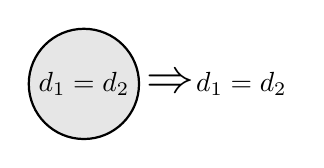
\begin{tikzpicture}[
    thick]
    \draw [fill=gray, fill opacity=0.2] (0,0) circle (.7cm);
    \draw (0,0) node {$d_1 = d_2$};
    \draw (1.1,0) node {\LARGE$\Rightarrow$};
    \draw (2,0) node {$d_1 = d_2$};
\end{tikzpicture}
      \caption{No Duplicates Rule}
    \end{subfigure}%
    \begin{subfigure}{.22\textwidth}
\vspace*{2.5em}
      \centering
\def\firstcircle{(0,0) circle (.7cm)}
\def\secondcircle{(.7,0) circle (.7cm)}
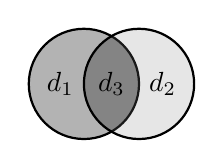
\begin{tikzpicture}[thick]
\begin{scope}
        \clip \firstcircle;
        \fill[fill=gray, fill opacity=0.9] \secondcircle;
\end{scope}
    \draw [fill=gray, fill opacity=0.6] \firstcircle;
    \draw (-0.3,0) node {$d_1$};
    \draw [fill=gray, fill opacity=0.2] \secondcircle;
    \draw (1.0,0) node {$d_2$};
    \draw (0.35,0) node {$d_3$};
\end{tikzpicture}
      \caption{Meet Rule}
    \end{subfigure}
    \begin{subfigure}{.5\textwidth}
	  \centering
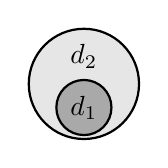
\begin{tikzpicture}[thick]
    \draw [fill=gray, fill opacity=0.2] (0,0) circle (.7cm);
    \draw [fill=gray, fill opacity=0.6] (0,-0.3) circle (.35cm);
    \draw (0,0.35) node {$d_2$};
    \draw (0,-0.3) node {$d_1$};
\end{tikzpicture}
\begin{tikzpicture}[thick]
    \draw (0,.45) node {\LARGE$\Rightarrow$};
\begin{pgflowlevelscope}{\pgftransformscale{.5}}
\node[fill=gray,fill opacity=0.2,draw,regular polygon,regular polygon sides=5,xshift=1.44cm,yshift=1.6cm,minimum size=12.4mm,outer sep=0] {};
\node[opacity=0,draw,circle,xshift=1.6cm,yshift=1.6cm,minimum size=10mm,outer sep=0] (bigtop) {};
\node[fill=gray,fill opacity=0.2,draw,regular polygon,regular polygon sides=5,yshift=1.6cm,xshift=7.0cm,minimum size=.5mm,outer sep=0] (smalltop) {};
\node[opacity=0,draw,circle,yshift=1.6cm,xshift=6.9cm,minimum size=1.0mm,outer sep=0] (smalltop) {};
\draw (tangent cs:node=bigtop,point={(smalltop.south)},solution=2) -- (tangent cs:node=smalltop,point={(bigtop.south)});
\draw (tangent cs:node=bigtop,point={(smalltop.north)},solution=1) -- (tangent cs:node=smalltop,point={(bigtop.north)},solution=2);
\end{pgflowlevelscope}
    \draw (0.5,1.8) node {{\footnotesize instances}};
    \draw (.83,1.5) node {{\footnotesize applicable to $\alpha$}};
    \draw (2.15,0.8) node {$\forall$};
    \draw (2.15,0.0) node {$\exists$};
    \draw (4.0,1.7) node {{\footnotesize return}};
    \draw (3.95,1.4) node {{\footnotesize types}};
    \draw (4.0,0.75) node {$\tau_2$};
    \draw (4.0,0.35) node {$\ddot{\vee}$};
    \draw (4.0,-0.05) node {$\tau_1$};
\begin{pgflowlevelscope}{\pgftransformscale{.5}}
\node[fill=gray, fill opacity=0.6,draw,regular polygon,regular polygon sides=5,xshift=1.44cm,minimum size=12.4mm,outer sep=0] {};
\node[opacity=0,draw,circle,minimum size=10mm,xshift=1.6cm,outer sep=0] (big) {};
\node[fill=gray,fill opacity=0.6,draw,draw,regular polygon,regular polygon sides=5,xshift=7.0cm,minimum size=1mm,outer sep=0] {};
\node[opacity=0.0,draw,circle,xshift=6.9cm,minimum size=1mm,outer sep=0] (small) {};
\draw (tangent cs:node=big,point={(small.south)},solution=2) -- (tangent cs:node=small,point={(big.south)});
\draw (tangent cs:node=big,point={(small.north)},solution=1) -- (tangent cs:node=small,point={(big.north)},solution=2);
\end{pgflowlevelscope}
    \draw (.75,0.8) node {{\footnotesize $d_2$}};
    \draw (0.75,0.0) node {{\footnotesize $d_1$}};
\end{tikzpicture}
	  \caption{Return Type Rule}
	\end{subfigure}
    \caption{Overloading rules for multiple inheritance and generics
where circles denote applicable sets of generic method declarations
and pentagons denote instantiated method declarations}
    \label{fig:overloading}
\end{figure}

The overloading rules of FGF require every pair in a set of
overloaded method declarations to satisfy \emph{all} of the following
rules as illustrated in Figure~\ref{fig:overloading}:
\begin{description}
\item[\textbf{No Duplicates Rule:}]
Distinct method declarations
must have different applicable sets
(there must be some argument type $\alpha$ for which one method is applicable and the other is not).

\item[\textbf{Meet Rule:}] Let $\mathcal{S}$ be the intersection of the applicable sets of the two method declarations;
if $\mathcal{S}$ is not empty, then the overloaded set must contain a method declaration
(not necessarily distinct from the two given method declarations) whose applicable set is precisely $\mathcal{S}$.

\item[\textbf{Return Type Rule:}] If one method declaration $d_1$ is
more specific than $d_2$, for any non-$\Bottom$ type $\alpha$ in the
applicable set of $d_1$, the return type of an instance of $d_2$ that is
applicable to $\alpha$ must be a supertype of the return type of
some instance of $d_1$ that is applicable to $\alpha$.
\end{description}

Let us revisit the above ambiguous $\mbox{\textit{sort}}$ example
with an additional method declaration:
\[\begin{array}[ht]{r@{\qquad}l}
d_1:&\mbox{\textit{sort}}\ob{P \extends A}(x \COLON \kwd{List^I}\ob{P}) \COLON \kwd{SortedList^I}\ob{P} = \cdots\\
d_2:&\mbox{\textit{sort}}\ob{P \extends B}(x \COLON \kwd{List^I}\ob{P}) \COLON \kwd{SortedList^I}\ob{P} = \cdots\\
d_3:&\mbox{\textit{sort}}\ob{P \extends C}(x \COLON \kwd{List^I}\ob{P}) \COLON \kwd{SortedList^I}\ob{P} = \cdots\\
\end{array}\]
% This set of overloaded method declarations is valid since every pair
% satisfies all of the above overloading rules.
This set of overloaded method declarations is valid.
For all pairs, the No Duplicates Rule is trivially satisfied.
In the case of $d_1$ and
$d_2$, the Meet Rule is satisfied
% by $d_3$ being the meet of this pair,
($d_3$ is their meet),
and the Return Type Rule is vacuously satisfied since neither is more specific than the other.
% In the case of
For
$d_1$ and $d_3$, the Meet Rule is satisfied with $d_3$ itself as the meet; to see that
the Return Type Rule is satisfied, note that $\kwd{List^I}$ is an invariant
type constructor since FGF does not support variance.  For any
$\kwd{List^I}\ob{X}$ in the applicable set of $d_3$, there is exactly one instance
of $d_1$ (with $X$ substituted for $P$) applicable to it:
\begin{center}
$\mbox{\textit{sort}}(x \COLON \kwd{List^I}\ob{X}) \COLON \kwd{SortedList^I}\ob{X} = \cdots$.
\end{center}
Since the return type of this instance equals the return type of the corresponding instance of $d_3$: 
\begin{center}
$\mbox{\textit{sort}}(x \COLON \kwd{List^I}\ob{X}) \COLON \kwd{SortedList^I}\ob{X} = \cdots$,
\end{center}
$d_1$ and $d_3$ satisfy the Return Type Rule.  Similarly, $d_2$ and $d_3$
also satisfy all of the overloading rules.

Again, the overloading rules ensure that there is no ambiguous method
calls at run time, and that types are preserved.  In FGF, No Duplicates
Rule rules out the trivial ambiguous calls with duplicate declarations.
Meet Rule plays an important role for ensuring the existence of a
disambiguating method declaration, and Return Type Rule serves a key
role for type preservation.


\subsection{Overloading Rules for Multiple Inheritance and Generics with Variance}
\label{sec:motiv:fgfv}
Variance, as well as symmetric multiple dispatch, multiple inheritance,
and generics, may cause ambiguous method calls that cannot be resolved
at run time.  We revisit the ambiguous $\mbox{\textit{sort}}$ example in
Section~\ref{sec:motiv:fgf}.  This time, we define the same method
in a simpler way using covariant definitions of $\kwd{List^C}$ and $\kwd{SortedList^C}$.
Consider the following overloaded method declarations of $\mbox{\textit{sort}}$:
\[\begin{array}[ht]{r@{\qquad}l}
d_1:&\mbox{\textit{sort}}(x \COLON \kwd{List^C}\ob{A}) \COLON \kwd{SortedList^C}\ob{A} = \cdots\\
d_2:&\mbox{\textit{sort}}(x \COLON \kwd{List^C}\ob{B}) \COLON \kwd{SortedList^C}\ob{B} = \cdots\\
\end{array}\]
Similarly to the example in Section~\ref{sec:motiv:fgf}, for a method invocation
$\mbox{\textit{sort}}(l)$ where the run-time type of $l$ is $\kwd{List^C}\ob{C}$,
it is ambiguous which declaration to invoke: both $d_1$ and
$d_2$ are applicable to $l$ and neither is more specific than the other.
In order to ensure that there is no ambiguous method calls for
$\mbox{\textit{sort}}$ at run time, we need to add a disambiguating method
declaration $d_3$:
\[\begin{array}[ht]{r@{\qquad}l}
d_3:&\mbox{\textit{sort}}(x \COLON \kwd{List^C}\ob{C}) \COLON \kwd{SortedList^C}\ob{C} = \cdots\\
\end{array}\]
with a more specific return type than those of $d_1$ and $d_2$ for type
preservation.
% Thus, overloading rules should consider generic types with variance as well to avoid any unambiguous method calls at run time.

Variance also adds complications in type-sound dynamic dispatch.  Let us now
assume that $\kwd{List^C}$ is covariant in its type argument but
$\kwd{SortedList^I}$ is invariant.
Then, the set of three method declarations above
replacing $\kwd{SortedList^C}$ with $\kwd{SortedList^I}$ would be invalid,
because the return type $\kwd{SortedList^I}\ob{A}$ of $d_1$ would not be a supertype of the return type $\kwd{SortedList^I}\ob{C}$ of $d_3$.

Supporting variance in a type-sound manner requires keeping
track of the static types of method invocations at run time.
Let us again assume that $\kwd{List^C}$ is covariant but $\kwd{SortedList^I}$ is invariant,
and consider the following overloaded set (note that $d_3$ now has a type parameter $P$):
\[\begin{array}[ht]{r@{\qquad}r}
d_1:&\mbox{\textit{sort}}(x \COLON \kwd{List^C}\ob{A}) \COLON \kwd{SortedList^I}\ob{A} = \cdots\\
d_2:&\mbox{\textit{sort}}(x \COLON \kwd{List^C}\ob{B}) \COLON \kwd{SortedList^I}\ob{B} = \cdots\\
d_3:&\mbox{\textit{sort}}\ob{P}(x \COLON \kwd{List^C}\ob{C}) \COLON \kwd{SortedList^I}\ob{P} = \cdots\\
\end{array}\]
as well as the following generic method declaration of $\mbox{\textit{merge}}$:
\begin{center}
$\mbox{\textit{merge}}\ob{P}(x \COLON \kwd{SortedList^I}\ob{P}, y \COLON \kwd{SortedList^I}\ob{P}) \COLON \kwd{SortedList^I}\ob{P} = \cdots$
\end{center}
For a method invocation
$\mbox{\textit{merge}}(\mbox{\textit{sort}}(l_1), \mbox{\textit{sort}}(l_2))$
where the static types of $l_1$ and $l_2$ are both $\kwd{List^C}\ob{A}$ and
their run-time types are $\kwd{List^C}\ob{A}$ and $\kwd{List^C}\ob{C}$, respectively,
at compile time, both method invocations $\mbox{\textit{sort}}(l_1)$ and
$\mbox{\textit{sort}}(l_2)$ choose $d_1$ and their static types are both
$\kwd{SortedList^I}\ob{A}$.  Thus, the above $\mbox{\textit{merge}}$ call
statically invokes the following instance of the generic
$\mbox{\textit{merge}}$ declaration:
\begin{center}
$\mbox{\textit{merge}}(x \COLON \kwd{SortedList^I}\ob{A}, y \COLON \kwd{SortedList^I}\ob{A}) \COLON \kwd{SortedList^I}\ob{A}$
\end{center}
that is applicable to $\tuple{\kwd{SortedList^I}\ob{A}, \kwd{SortedList^I}\ob{A}}$.
However, at run time, while $\mbox{\textit{sort}}(l_1)$ chooses $d_1$ and
its return type is $\kwd{SortedList^I}\ob{A}$, $\mbox{\textit{sort}}(l_2)$
chooses $d_3$ and its return type depends on what actual type is inferred at run time for the type parameter $P$.
If the dynamic type inference algorithm instantiates $P$ as $A$,
$\mbox{\textit{sort}}(l_2)$ has type $\kwd{SortedList^I}\ob{A}$, which is
type sound.  But it could equally plausibly instantiate $P$ as some other type $T$,
and then no dynamic instance of the generic $\mbox{\textit{merge}}$
declaration would be applicable to 
$\tuple{\kwd{SortedList^I}\ob{A}, \kwd{SortedList^I}\ob{T}}$.
Hence, the $\mbox{\textit{merge}}$ call would fail, despite the fact that
the program successfully passed static type checking.
In order to help run-time type inference
algorithms make type-sound choices of type arguments, the language
semantics needs to make the static types of method invocations available at run time.

In this paper, we present FGFV, which sheds light on the long-standing
endeavor to support strong types, symmetric multiple dispatch, multiple inheritance,
and parametric polymorphism with variance.
% Unlike existing approaches, FGFV captures only the core language features
% to address the problem, we formally define the FGFV calculus from its
% syntax, static semantics, and dynamic semantics, and we finally prove its
% type soundness.
We formalize the static overloading rules for FGFV using
existential types and universal types quantified over method type
parameters, and design a new dynamic dispatch algorithm that is proven
type-sound to guarantee unambiguous method calls and type preservation
at run time.

